As the goal is to attempt to verify the Jeffrey equations in eq \ref{eq:jeffrey} we need an experimental setup with 
particles and flow system that satisfy the conditions that the Jeffrey equations apply under. This means our particles 
have to be buoyant, triaxially symmetric and small enough that inertial effects are negligible. The flow has to be a 
linear creeping flow, in other words have a Reynolds number satisfying $Re << 1$ and have a high unidirectional shear 
that allows one to detect the orbits in a relatively short distance.


The particles used in previous measurements were made from apoxy mixed in a vortex\cite{JonasExperiment} which made 
them buoyant and small enough to ignore inertial effects, but they were not symmetrical enough to produce reliable 
periodic Jeffrey orbits. Thus two sets of glass particles from Nippon Glass, Japan\cite{Particles}, have been used. 
They are cylindrical with a consistent width of \unit[3]{$\mu$m} and \unit[5]{$\mu$m} and varying length. Images taken 
with a STEM microscope can be seen in figure \ref{fig:particlepictures}. 


\begin{figure}[H]
\centering
\begin{subfigure}[3a]{0.40\textwidth}
\includegraphics[width=\textwidth]{figures/method/semizoomed.png}
\caption{Shows a detailed view \\ of a number of particles.}
\end{subfigure}\hspace{1em}%
\begin{subfigure}[3b]{0.40\textwidth}
\includegraphics[width=\textwidth]{figures/method/zoomedbroken.png}
\caption{Shows in detail the jagged edge \\ of a particle.}
\end{subfigure}
\caption{Pictures of the glass particles that particles}
\label{fig:particlepictures}
\end{figure}


While these particles seemingly satisfy the symmetry conditions they are made glass with a density of approximately \unit[2.57]{g/cm$^3$} at \unit[20]{C$^\circ$} which is significantly higher than that of water with a density of \unit[1]{g/cm$^3$} at \unit[20]{C$^\circ$} and glycerol with a density of \unit[1.5]{g/cm$^3$}. Thus to correct for the density and limit sinking or floating the water soluble Sodium metatungstate which at \unit[20]{C$^\circ$} has maximum density of \unit[2.94]{g/cm$^3$}. To increase the viscosity of the liquid around 8\% glycerol is added, resulting in a measured dynamic viscosity of \unit[$24\cdot 10^{-3}$]{Pa s}

% PIcture of the channel meassurements here 
\begin{figure}[H]
\centering
%\begin{subfigure}
\includegraphics[width=0.7\textwidth]{figures/method/ChannelZoomed.jpg}
%\end{subfigure}
\end{figure}


This liquid with suspended particles is flowed through a channel of Polydimethylsiloxane (PDMS) \unit[4]{cm} long,
 \unit[2.5]{mm} wide and either \unit[200]{$\mu$m} and \unit[500]{$\mu$m}. The flow profile of such a channel was 
 calculated by Anton Johansson in his thesis\cite{AntonThesis} and can be seen in figure \ref{fig:flowprofile}. The 
 flow rate varies  between $2$ and \unitfrac[20]{$\mu$l}{m} or in SI units \unitfrac[$3.33\cdot 10^-10$]{m$^3$}{s} 
 which with a cross section of at least \unit[$5\cdot 10^-7$]{m$^2$}means a maximum flow speed of  
 \unitfrac[6.66]{mm}{s}.

% Picture of channel flow profile
\begin{figure}[H]
\begin{center}
\includegraphics[width=0.7\textwidth]{figures/method/flowprofile.pdf}
\end{center}
\caption{}
\label{fig:flowprofile}
\end{figure}

            
To confirm that the flow is a creeping flow we can calculate the maximum Reynolds number using eq \ref{eq:reynolds} and our maximum flow speed 

\begin{equation}
Re = \frac{U L \rho}{\mu} 
\leq \frac{6.66\cdot 10^{-3} \cdot 2.5 \cdot 10^{-3} 2.5 }{24 \cdot 10^{-3}} 
\approx	 	1.6  \cdot 10^{-3} \ll 1
\end{equation}

This should satisfy the conditions of the Jeffrey equations. To track the particles the channel is put in a moveable stage on a confocal microscope. The entire setup can be seen in figure \ref{fig:experimentalsetup}

%\begin{figure}
%\begin{center}
%\includegraphics[width=0.7\textwidth]{figures/setupsketch.png}
%\end{center}
%\caption{}
%\label{fig:experimentalsetup}
%\end{figure}

\begin{figure}[H]
\centering
\begin{subfigure}[b]{0.45\textwidth}
\includegraphics[width=0.9\textwidth]{figures/method/setupsketch.png}
\caption{Sketch of the set up}\label{fig:setupsketch}
\end{subfigure}
\begin{subfigure}[b]{0.45\textwidth}
\includegraphics[width=0.9\textwidth]{figures/method/ExperimentalOverview.jpg}
\caption{Overview of the set up}\label{fig:setuppicture}
\end{subfigure}
\caption{}
\label{fig:experimentalsetup}
\end{figure}

\begin{itemize}
\item 
\end{itemize}


\subsection{Density matching}


\begin{equation}
\rho_{a} = 	\frac {m_{a}}{V_{a}} =
				\frac{V_{b}\rho_{b} + V_{mix}\rho_{mix}}{V_b + V_{mix}} 
\end{equation}
So if we want to find $V_{mix}$ we get
\begin{equation}
V_{mix} = \frac{ V_{b}(\rho_{b} - \rho_{a})}{\rho_{a} - \rho_{mix}} 
\end{equation}

